\documentclass{article}

\usepackage{tikz}
\usetikzlibrary{calc}
\usetikzlibrary{positioning}

\usepackage{amssymb}


% Now we define the global styles

% We start by defining the default colours of vertices, edges and faces
\newcommand{\vertexColor}{blue}
\newcommand{\edgeColor}{black}
\newcommand{\faceColor}{yellow}

\newcommand{\vSize}{2.5pt}    % How big are the vertex circles (if drawn)?
% Command to set the vertex labels (in the correct colour)

\newcommand{\drawEdge}[3]{            
	\node[edgeBackground] at ($1/2*(#1)+1/2*(#2)$) {#3};
}


\tikzset{vertex/.style = {\vertexColor}}
\tikzset{edge/.style = {\edgeColor, thick}}
\tikzset{edgeBackground/.style = {fill=blue!20!white}}
\tikzset{face/.style = {fill=\faceColor, draw=\edgeColor}}


\begin{document}

              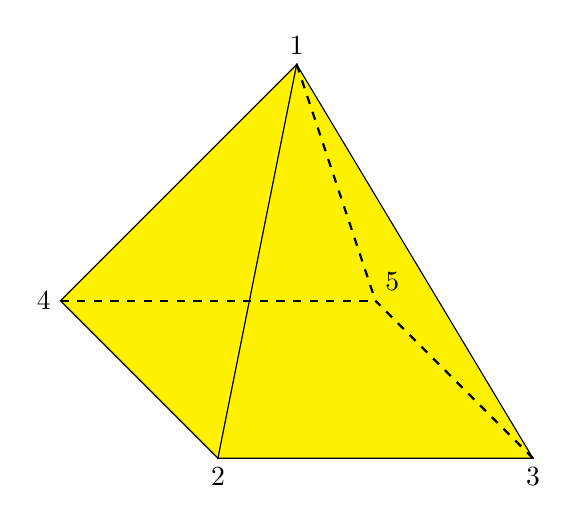
\begin{tikzpicture}
                    \def\len{4}
                    \def\h{1}
                    \coordinate [label=above:1] (A) at (0.25*\len,0.25*\len+\len*\h);
                    \coordinate [label=below:2] (B) at (0,0);
                    \coordinate [label=below:3] (C) at (\len,0);
                    \coordinate [label=left:4] (D) at (-0.5*\len,0.5*\len);
                    \coordinate [label=right:5] (E) at ($(C)+(D)$);

                    \filldraw[face] (A) -- (B) -- (D) -- cycle;
                    \filldraw[face] (A) -- (B) -- (C) -- cycle;

                    \draw[edge, dashed] (D) -- (E);
                    \draw[edge, dashed] (C) -- (E);
                    \draw[edge, dashed] (A) -- (E);
                    % We have to rewrite this label as it is behind the pyramid
                    \node[above right] at (E) {5};
                \end{tikzpicture}
 

\end{document} 